% FUSAO (26/10/2026): float copied unchanged from tables_C*.tex, tables_main.tex or tables_appendix.tex.
\begin{figure}[htbp]\centering
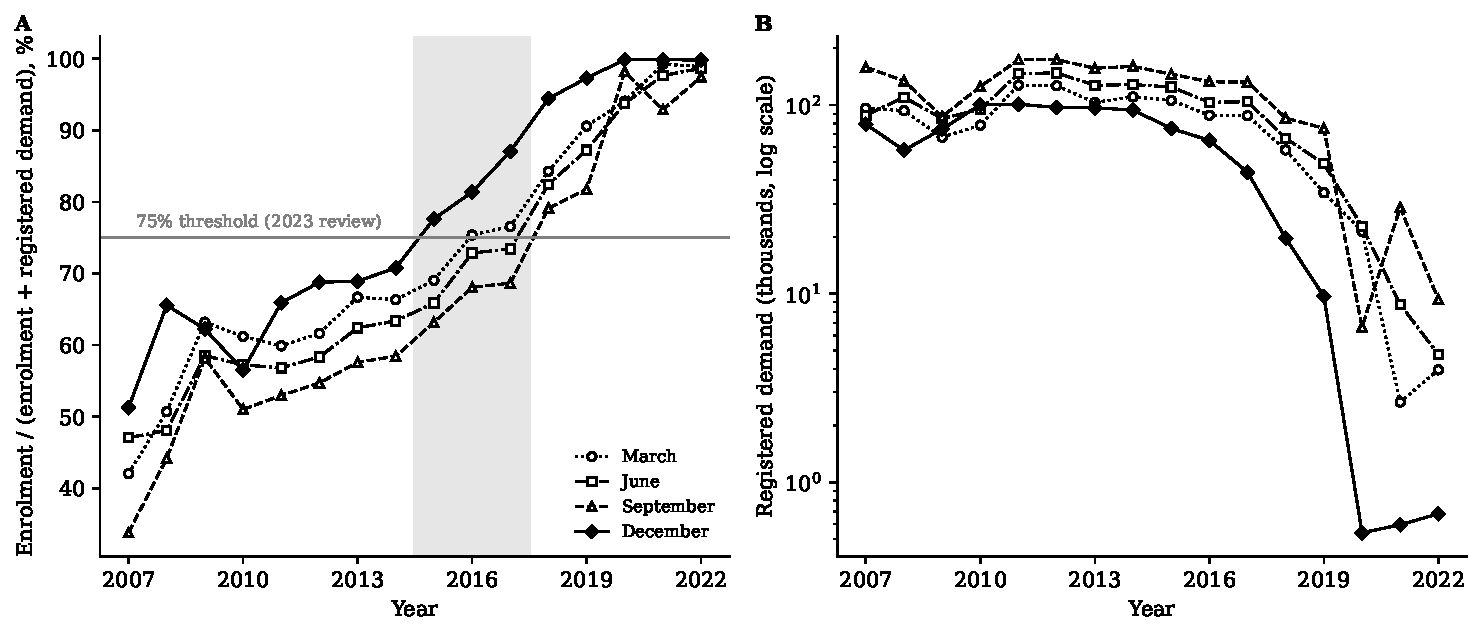
\includegraphics[width=\textwidth]{C_fig_goal}
\caption{Share of registered children served and registered demand in S\~ao Paulo, by reporting month, 2007--2022}
\label{fig:goal}
% Texto anterior, redigido com IA e fora de uso: _arquivo_texto_IA_2026-10-27/legendas_notas_corpo/V3w_fig_goal.tex
\tabnote{\emph{Sources:} Municipal Secretariat of Education (SME), published series of childcare enrolment and registered demand. Panel A reports childcare enrolment as a percentage of the sum of enrolment and registered demand. The horizontal line marks the 75\% threshold used in the 2023 review. The shaded interval identifies 2015--2017, when the December count met this threshold but the September count did not. Panel B reports registered demand in thousands of children on a logarithmic scale. Both panels distinguish the March, June, September and December counts, with the same series identification throughout. The series end in 2022, the last year for which all four counts are available. Registered demand measures recorded applications awaiting a place rather than the full population of children without access to childcare.}
\par\smallskip\noindent\begin{minipage}{\linewidth}\footnotesize\raggedright Alt text: Two-panel line chart covering 2007--2022, with four series corresponding to March, June, September and December observations. Panel A plots the percentage of registered children served, with a horizontal reference line at 75\% and shading over 2015--2017. Panel B plots registered demand in thousands of children on a logarithmic scale.\end{minipage}
\end{figure}
